\documentclass{standalone}

\usepackage[euler-digits]{eulervm}

\usepackage{tikz}
\tikzset{every node/.style={circle,draw,minimum size=6mm,inner sep=0pt}}
\tikzset{t/.style={rectangle}}

\begin{document}
    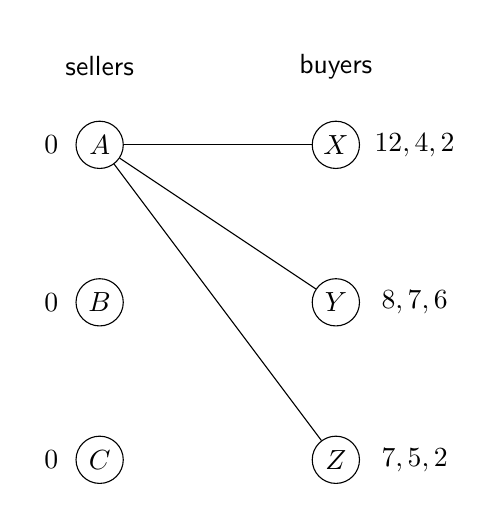
\begin{tikzpicture}[font=\sffamily]
        \node[draw=none] (S) at (-1,5) {sellers};
        \node[draw=none] (B) at (2,5) {buyers};
%        \node[draw=none] (B) at (3,5) {valuations};
      \node[label=left:{$0$}] (A) at (-1,4) {$A$}; 
      \node[label=left:{$0$}] (B) at (-1,2) {$B$}; 
      \node[label=left:{$0$}] (C) at (-1,0) {$C$}; 
      \node (X) at (2,4) {$X$}; 
      \node[draw=none] (V1) at (3,4) {$12,4,2$};
      \node (Y) at (2,2) {$Y$}; 
      \node[draw=none] (V2) at (3,2) {$8,7,6$};
      \node (Z) at (2,0) {$Z$}; 
      \node[draw=none] (V3) at (3,0) {$7,5,2$};
      \foreach \a/\b in {A/X,A/Y,A/Z}
        \draw (\a) -- (\b);
    \end{tikzpicture}
\end{document}
